\documentclass{standalone}

\usepackage{tikz}
\usetikzlibrary{calc}
\usetikzlibrary{bayesnet}



\begin{document}

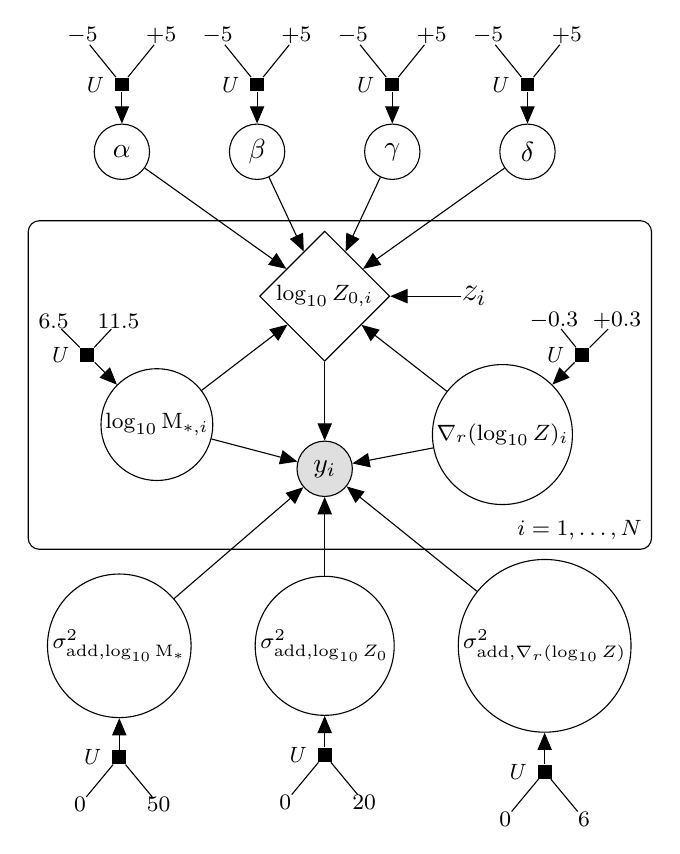
\begin{tikzpicture}

    \node[latent] (beta) {$\beta$} ;  %
    \node[latent, left=of beta] (alpha)  {$\alpha$} ;  %
	\node[latent, right=of beta] (gamma) {$\gamma$} ; %
	\node[latent, right=of gamma] (delta) {$\delta$} ; %
	\coordinate (beta_gamma) at ($ (beta) !.5! (gamma) $) ;  %
	
	\node[det, below=of beta_gamma] (logZ0) {\footnotesize $\log_{10}Z_{0,i}$} ; %
	\node[latent, below left=of logZ0, xshift=-0.5cm] (mass) {\footnotesize $\log_{10}{\rm M}_{\ast,i}$} ; %
	\node[latent, below right=of logZ0, xshift=+0.5cm] (dlogZ) {\footnotesize $\nabla_r(\log_{10}Z)_i$} ; %
    \node[const, right=0.9 of logZ0] (z) {\large $z_i$} ; %	
	
	\node[obs, below=of logZ0] (obs) {$y_i$} ; %

	\node[latent, below=of obs] (err_logZ0) {\footnotesize $\sigma^2_{\mathrm{add},\log_{10}Z_0}$} ; %
	\node[latent, left=of err_logZ0, xshift=0.2cm] (err_mass) {\footnotesize $\sigma^2_{\mathrm{add},\log_{10}{\rm M}_\ast}$} ; %
	\node[latent, right=of err_logZ0, xshift=-0.2cm] (err_dlogZ) {\footnotesize $\sigma^2_{\mathrm{add},\nabla_r(\log_{10}Z)}$} ; %

    \edge {alpha} {logZ0} ; %
	\edge {beta} {logZ0} ; %
    \edge {gamma} {logZ0} ; %
    \edge {delta} {logZ0} ; %

    \edge {mass} {logZ0} ; %
    \edge {dlogZ} {logZ0} ; %
    \edge {z} {logZ0} ; %


    \edge {mass} {obs} ; %
    \edge {logZ0} {obs} ; %
    \edge {dlogZ} {obs} ; %

    \edge {err_mass} {obs} ; %
    \edge {err_logZ0} {obs} ; %
    \edge {err_dlogZ} {obs} ; %

    \node[const, above=of alpha, xshift=-0.5cm] (alpha_min) {\footnotesize $-5$} ; %
    \node[const, above=of alpha, xshift=+0.5cm] (alpha_max) {\footnotesize $+5$} ; %
    \node[const, above=of beta, xshift=-0.5cm] (beta_min) {\footnotesize $-5$} ; %
    \node[const, above=of beta, xshift=+0.5cm] (beta_max) {\footnotesize $+5$} ; %
    \node[const, above=of gamma, xshift=-0.5cm] (gamma_min) {\footnotesize $-5$} ; %
    \node[const, above=of gamma, xshift=+0.5cm] (gamma_max) {\footnotesize $+5$} ; %
    \node[const, above=of delta, xshift=-0.5cm] (delta_min) {\footnotesize $-5$} ; %
    \node[const, above=of delta, xshift=+0.5cm] (delta_max) {\footnotesize $+5$} ; %
    
    
    \factor[above=of alpha] {alpha_dist} {left:$\mathit{U}$} {alpha_min,alpha_max} {alpha} ; % 
    \factor[above=of beta] {beta_dist} {left:$\mathit{U}$} {beta_min,beta_max} {beta} ; %
    \factor[above=of gamma] {gamma_dist} {left:$\mathit{U}$} {gamma_min,gamma_max} {gamma} ; %
    \factor[above=of delta] {delta_dist} {left:$\mathit{U}$} {delta_min,delta_max} {delta} ; %

    \node[const, above left=of mass, xshift=+0.1cm] (mass_min) {\footnotesize $6.5$} ; %
    \node[const, above left=of mass, xshift=+1cm] (mass_max) {\footnotesize $11.5$} ; %
    \node[const, above right=of dlogZ, xshift=-1cm] (dlogZ_min) {\footnotesize $-0.3$} ; %
    \node[const, above right=of dlogZ,, xshift=-0.2cm] (dlogZ_max) {\footnotesize $+0.3$} ; %

    \factor[above left=of mass] {mass_dist} {left:$\mathit{U}$} {mass_min,mass_max} {mass} ; % 
    \factor[above right=of dlogZ] {dlogZ_dist} {left:$\mathit{U}$} {dlogZ_min,dlogZ_max} {dlogZ} ; % 

    \node[const, below=of err_mass, xshift=-0.5cm] (err_mass_min) {\footnotesize $0$} ; %
    \node[const, below=of err_mass, xshift=+0.5cm] (err_mass_max) {\footnotesize $50$} ; %
    \node[const, below=of err_logZ0, xshift=-0.5cm] (err_logZ0_min) {\footnotesize $0$} ; %
    \node[const, below=of err_logZ0, xshift=+0.5cm] (err_logZ0_max) {\footnotesize $20$} ; %
    \node[const, below=of err_dlogZ, xshift=-0.5cm] (err_dlogZ_min) {\footnotesize $0$} ; %
    \node[const, below=of err_dlogZ, xshift=+0.5cm] (err_dlogZ_max) {\footnotesize $6$} ; %

    \factor[below=of err_mass] {err_mass_dist} {left:$\mathit{U}$} {err_mass_min,err_mass_max} {err_mass} ; % 
    \factor[below=of err_logZ0] {err_logZ0_dist} {left:$\mathit{U}$} {err_logZ0_min,err_logZ0_max} {err_logZ0} ; % 
    \factor[below=of err_dlogZ] {err_dlogZ_dist} {left:$\mathit{U}$} {err_dlogZ_min,err_dlogZ_max} {err_dlogZ} ; % 


	\plate {plate} { %
   		(mass_min) (mass_max) (mass_dist) (mass) (logZ0) (dlogZ) (dlogZ_min) (dlogZ_max) (dlogZ_dist) (z) (obs) %
	    } {$i = 1, \ldots, N$}; 

\end{tikzpicture}

\end{document}
